\section{Proofs}
\label{app:proof}

\subsection{WA loss derivation}
\label{app:wa_loss}
\begin{lemma*}[\ref{lemma:wa_ensembling}]
    Given $\{\theta_m\}_{m=1}^M$ with learning procedures $L_S^M\triangleq\{l_S^{(m)}\}_{m=1}^M$. Denoting $\Delta_{L_S^M}=\max_{m=1}^{M}\left\|\theta_m-\theta_{\text{WA}}\right\|_2$, $\forall (x,y) \in \X \times \Y$:%
    \begin{equation*}
        f_{\text{WA}}(x) = f_{\text{ENS}}(x) + O(\Delta^2_{L_S^M}) \text{~and~} \ell\left(f_{\text{WA}}(x), y\right) = \ell\left(f_{\text{ENS}}(x) , y\right) + O(\Delta_{L_S^M}^2).%
    \end{equation*}%
\end{lemma*}
\begin{proof}
This proof has two components:
\begin{itemize}
    \item to establish the functional approximation, as \cite{izmailov2018}, it performs Taylor expansion of the models' predictions at the first order.
    \item to establish the loss approximation, as \cite{Wortsman2022ModelSA}, it performs Taylor expansion of the loss at the first order.
\end{itemize}
% \footnote{at the first order instead of the second order in \cite{Wortsman2022ModelSA}.}
\paragraph{Functional approximation}
With a Taylor expansion at the first order of the models' predictions \wrt parameters $\theta$:
\begin{align*}
    f_{\theta_m}&=f_{\text{WA}}+\nabla f_{\text{WA}}^\intercal \Delta_m+ O\left(\left\|\Delta_m\right\|_2^2\right)\\
    f_{\text{ENS}}-f_{\text{WA}}&=\frac{1}{M} \sum_{m=1}^{M}\left(\nabla f_{\text{WA}}^\intercal \Delta_m+O\left(\left\|\Delta_m\right\|_2^{2}\right)\right)
\end{align*}
Therefore, because $\sum_{m=1}^{M} \Delta_m=0$,
\begin{equation} \label{eq:diff_fens_fwa}
    f_{\text{ENS}}-f_{\text{WA}} = O\left(\Delta^2\right) \text{~where~}\Delta=\max_{m=1}^{M}\left\|\Delta_m\right\|_2.
\end{equation}
\paragraph{Loss approximation}
With a Taylor expansion at the zeroth order of the loss \wrt its first input and injecting \Cref{eq:diff_fens_fwa}:
\begin{align*}
    \ell\left(f_{\text{ENS}}(x) ; y\right)&=\ell\left(f_{\text{WA}}(x); y\right)+O\left(\left\|f_{\text{ENS}}(x)-f_{\text{WA}}(x)\right\|_2\right) \\
     \ell\left(f_{\text{ENS}}(x) ; y\right) &= \ell\left(f_{\text{WA}}(x); y\right) + O\left(\Delta^2\right).
\end{align*}
\end{proof}
\subsection{Bias-variance-covariance-locality decomposition}

\begin{remark} \label{remark:identical_assumption}
    Our result in \Cref{prop:b_var_cov} is simplified by leveraging the fact that the learning procedures $L_S^M=\{l_S^{(m)}\}_{m=1}^M$ are identically distributed (i.d.). This assumption naturally holds for DiWA which selects weights from different runs with i.i.d. hyperparameters.
    It may be less obvious why it applies to MA \cite{arpit2021ensemble} and SWAD \cite{cha2021wad}.
    It is even false if the weights $\{\theta(l_S^{(m)})\}_{m=1}^M$ are defined as being taken sequentially along a training trajectory, \ie when $0\leq i < j \leq M$ implies that $l_S^{(i)}$ has fewer training steps than $l_S^{(j)}$.
    We propose an alternative indexing strategy to respect the i.d. assumption.
    Given $M$ weights selected by the weight selection procedure, we draw without replacement the $M$ weights, \ie $\theta(l_S^{(i)})$ refers to the $i^{th}$ sampled weights.
    With this procedure, all weights are i.d. as they are uniformly sampled.
    Critically, their WA are unchanged for the two definitions.%
\end{remark}
\label{app:proof_bvc}
\begin{proposition*}[\ref{prop:b_var_cov}]
    Denoting $\bar{f}_S\left(x\right) = \mathbb{E}_{l_S} \left[f\left(x,\theta\left(l_S\right)\right)\right]$, under identically distributed learning procedures $L_S^M\triangleq\{l_S^{(m)}\}_{m=1}^M$, the expected generalization error on domain $T$ of $\theta_{\text{WA}}(L_S^M)\triangleq\frac{1}{M} \sum\nolimits_{m=1}^{M} \theta_m$ over the joint distribution of $L_S^M$ is:%
    \begin{equation*}\tag{\ref{eq:b_var_cov}}
        \begin{aligned}
             \mathbb{E}_{L_S^M}\mathcal{E}_T(\theta_{\text{WA}}(L_S^M)) &= \mathbb{E}_{(x,y)\sim p_T}\Big[\biasb^2(x, y)+\frac{1}{M} \varb(x)+\frac{M-1}{M} \covb(x)\Big] + O(\Deltab^2), \\
             \text{where~}\biasb(x,y)&=y-\bar{f}_S\left(x\right), \\
             \text{and~}\varb(x)&=\mathbb{E}_{l_S}\left[\left(f(x, \theta(l_S)) - \bar{f}_S\left(x\right)\right)^{2}\right], \\
             \text{and~}\covb(x)&= \mathbb{E}_{l_S,l_S'}\left[\left(f(x,\theta(l_S))-\bar{f}_S\left(x\right)\right)\left(f(x,\theta(l_S')))-\bar{f}_S\left(x\right)\right)\right], \\
             \text{and~}\Deltab^2&=\mathbb{E}_{L_S^M}\Delta_{L_S^M}^2 \text{~with~} \Delta_{L_S^M}=\max_{m=1}^{M}\left\|\theta_m-\theta_{\text{WA}}\right\|_2.%
        \end{aligned}%
    \end{equation*}%
    $\covb$ is the prediction covariance between two member models whose weights are averaged.
    The locality term $\Deltab^2$ is the expected squared maximum distance between weights and their average.
\end{proposition*}
\begin{proof}
    This proof has two components:
    \begin{itemize}
        \item it follows the bias-variance-covariance decomposition from \cite{ueda1996generalization,brown2005between} for functional ensembling. It is tailored to WA by assuming that learning procedures are identically distributed.
        \item it injects the obtained equation into \Cref{lemma:wa_ensembling} to obtain the \Cref{prop:b_var_cov} for WA.
    \end{itemize}
    \paragraph{BVC for ensembling with identically distributed learning procedures}
    With $\bar{f}_S\left(x\right) = \mathbb{E}_{l_S} \left[f\left(x,\theta\left(l_S\right)\right)\right]$, we recall the bias-variance decomposition \cite{kohavi1996bias} (\Cref{eq:b_v}):
    \begin{align*}
        \mathbb{E}_{l_S}\mathcal{E}_T(\theta(l_S)) & = \mathbb{E}_{(x,y)\sim p_T}\Big[\biasb(x,y)^{2}+\varb(x)\Big],\\
        \text{where~}\biasb(x,y) & =  \operatorname{Bias}\{f|(x,y)\} = y-\bar{f}_S\left(x\right), \\
        \text{and~}\varb(x) &= \operatorname{Var}\{f|x\} = \mathbb{E}_{l_S}\left[\left(f(x, \theta(l_S)) - \bar{f}_S\left(x\right)\right)^{2}\right]. \\
    \end{align*}
    Using $f_{\text{ENS}}\triangleq f_{\text{ENS}}(\cdot, \{\theta(l_S^{(m)})\}_{m=1}^M) \triangleq \frac{1}{M} \sum_{m=1}^{M} f(\cdot, \theta(l_S^{(m)}))$ in this decomposition yields,
    \begin{equation} \label{eq:b_v_ens}
        \mathbb{E}_{L_S^M}\mathcal{E}_T(\{\theta(l_S^{(m)})\}_{m=1}^M)=\mathbb{E}_{x\sim p_T}\left[\operatorname{Bias}\left\{f_{\text{ENS}} \mid (x,y)\right\}^{2}+\operatorname{Var}\left\{f_{\text{ENS}} \mid x\right\}\right].
    \end{equation}
    As $f_{\text{ENS}}$ depends on $L_S^M$, we extend the bias into:
    \begin{align*}
        \operatorname{Bias}\left\{f_{\text{ENS}} \mid (x,y)\right\}&=y-\mathbb{E}_{L_S^M}\left[\frac{1}{M} \sum_{m=1}^{M} f(x, \theta(l_S^{(m)}))\right]=y-\frac{1}{M} \sum_{m=1}^{M} \mathbb{E}_{l_S^{(m)}}\left[f(x, \theta(l_S^{(m)}))\right]
    \end{align*}
    Under identically distributed $L_S^M\triangleq\{l_S^{(m)}\}_{m=1}^M$,
    $$
        \frac{1}{M} \sum_{m=1}^{M} \mathbb{E}_{l_S^{(m)}}\left[y-f(x, \theta(l_S^{(m)}))\right]=\mathbb{E}_{l_S}\left[y-f(x, \theta(l_S))\right]=\operatorname{Bias}\{f|(x,y)\}.
    $$
    Thus the bias of ENS is the same as for a single member of the WA.
    
    Regarding the variance:
    \begin{align*}
        &\operatorname{Var}\left\{f_{\text{ENS}} \mid x\right\}=\mathbb{E}_{L_S^M}\left[\left(\frac{1}{M} \sum_{m=1}^{M} f(x, \theta(l_S^{(m)}))-\mathbb{E}_{L_S^M}\left[\frac{1}{M} \sum_{m=1}^{M} f(x, \theta(l_S^{(m)}))\right]\right)^{2}\right].\\
        % &=\frac{1}{M^{2}} \sum_{m=1}^{M} \mathbb{E}_{l_S^{(m)}}\left[\left(f(x, \theta(l_S^{(m)}))-\mathbb{E}_{l_S^{(m)}}\left[f(x, \theta(l_S^{(m)}))\right]\right)^{2}\right]+ \\
        % &\quad\quad \frac{1}{M^{2}} \sum_{m} \sum_{m^{\prime} \neq m} \mathbb{E}_{l_S^{(m)}, l_S^{(m^{\prime})}}[\left(f(x, \theta(l_S^{(m)}))-\mathbb{E}_{l_S^{(m)}}\left[f(x, \theta(l_S^{(m)}))\right]\right) \\
        % & \left(f(x, \theta(l_S^{(m^\prime)}))-\mathbb{E}_{l_S^{(m^{\prime})}}\left[f(x, \theta(l_S^{(m^\prime)}))\right]\right)].
    \end{align*}
    Under identically distributed $L_S^M\triangleq\{l_S^{(m)}\}_{m=1}^M$,
    \begin{align*}
        &\operatorname{Var}\left\{f_{\text{ENS}} \mid x\right\} = \frac{1}{M^{2}} \sum_{m=1}^{M} \mathbb{E}_{l_S}\left[\left(f(x, \theta(l_S))-\mathbb{E}_{l_S}\left[f(x, \theta(l_S))\right]\right)^{2}\right]+ \\
        &\quad\quad\quad\quad \frac{1}{M^{2}} \sum_{m} \sum_{m^{\prime} \neq m} \mathbb{E}_{l_S, l_S^\prime}\left[\left(f(x, \theta(l_S))-\mathbb{E}_{l_S}\left[f(x, \theta(l_S))\right]\right)\left(f(x, \theta(l_S^\prime))-\mathbb{E}_{l_S^\prime}\left[f(x, \theta(l_S^\prime))\right]\right)\right] \\
        &= \frac{1}{M} \mathbb{E}_{l_S}\left[\left(f(x, \theta(l_S))-\mathbb{E}_{l_S}\left[f(x, \theta(l_S))\right]\right)^{2}\right] + \\
        &\quad\quad\quad\quad \frac{M-1}{M}\mathbb{E}_{l_S, l_S^\prime}\left[\left(f(x, \theta(l_S))-\mathbb{E}_{l_S}\left[f(x, \theta(l_S))\right]\right)\left(f(x, \theta(l_S^\prime))-\mathbb{E}_{l_S^\prime}\left[f(x, \theta(l_S^\prime))\right]\right)\right] \\
        &=\frac{1}{M} \varb\left(x\right)+\left(1-\frac{1}{M}\right) \covb\left(x\right).
    \end{align*}
    The variance is split into the variance of a single member (divided by $M$) and a covariance term.
    \paragraph{Combination with \Cref{lemma:wa_ensembling}}
    We recall that per \Cref{lemma:wa_ensembling},
    \begin{align*}
        \ell\left(f_{\text{WA}}(x), y\right) = \ell\left(f_{\text{ENS}}(x) , y\right) + O(\Delta_{L_S^M}^2).
    \end{align*}
    Then we have:
    \begin{align*}
        \mathcal{E}_T(\theta_{\text{WA}}(L_S^M))&=\mathbb{E}_{(x,y) \sim p_T}[\ell(f_{\text{WA}}(x),y)]\\
        &=\mathbb{E}_{(x,y) \sim p_T}[\ell(f_{\text{ENS}}(x),y)] + O(\Delta_{L_S^M}^2) = \mathcal{E}_T(\{\theta(l_S^{(m)})\}_{m=1}^M) + O(\Delta_{L_S^M}^2), \\
        \mathbb{E}_{L_S^M} \mathcal{E}_T(\theta_{\text{WA}}(L_S^M))&=\mathbb{E}_{L_S^M}\mathcal{E}_T(\{\theta(l_S^{(m)})\}_{m=1}^M) + O(\mathbb{E}_{L_S^M}[\Delta_{L_S^M}^2]).
    \end{align*}
    We eventually obtain the result:
    \begin{align*}
        % \mathcal{E}_T(\theta_{\text{WA}}(L_S^M)) =
        \mathbb{E}_{L_S^M}\mathcal{E}_T(\theta_{\text{WA}}(L_S^M)) = \mathbb{E}_{(x,y)\sim p_T}\Big[\biasb(x,y)^{2}+\frac{1}{M} \varb(x)+\frac{M-1}{M} \covb(x)\Big] + O(\Deltab^2).
    \end{align*}
\end{proof}%
\subsection{Bias, correlation shift and support mismatch}
\label{app:bias_correlation}
We first present in \Cref{app:app_bias_full} a decomposition of the \ood bias without any assumptions.
We then justify in \Cref{app:bias_correlation_ass_noiidbias} the simplifying \Cref{ass:no_bias_iid} from \Cref{subsec:expression_ood_bias}.
\subsubsection{\ood bias}
\label{app:app_bias_full}
\begin{proposition}[\ood bias]
    \label{prop:app_bias_full}
    Denoting $\bar{f}_{S}\left(x\right) = \mathbb{E}_{l_S}[f\left(x,\theta\left(l_S\right)\right)]$, the bias is:
    \begin{align*}
        &\mathbb{E}_{(x,y)\sim p_T} [\biasb^2(x, y)] = \int_{\X_T \cap \X_S} \left(f_T\left(x\right)-f_S\left(x\right)\right)^{2} p_T(x) dx                                          & (\text{Correlation shift})                                               \\
                         & + \int_{\X_T \cap \X_S} \left(f_{S}(x)-\bar{f}_{S}\left(x\right)\right)^{2} p_T(x) dx                                                            & (\text{Weighted \iid bias})                                               \\
                         & + \int_{\X_T \cap \X_S} 2 \left(f_T\left(x\right) - f_S\left(x\right)\right) \left(f_S\left(x\right) - \bar{f}_{S}\left(x\right)\right) p_T(x)dx & (\text{Interaction \iid bias and corr. shift})                     \\
                         & + \int_{\X_T \setminus \X_S} \left(f_T\left(x\right)-\bar{f}_{S}\left(x\right)\right)^{2} p_T(x) dx.                                   & (\text{Support mismatch}) %
    \end{align*}%
\end{proposition}%

\begin{proof}
    This proof is original and based on splitting the \ood bias in and out of $\X_S$:
    \begin{align*}
        &\mathbb{E}_{(x,y)\sim p_T}[\biasb^2(x, y)] = \mathbb{E}_{(x,y)\sim p_T} \left(y -\bar{f}_{S}\left(x\right)\right)^{2}                          \\
                                         & = \int_{\X_T} \left(f_T\left(x\right)-\bar{f}_{S}\left(x\right)\right)^{2} p_T(x) dx                \\
                                         & =\int_{\X_T \cap \X_S} \left(f_T\left(x\right)-\bar{f}_{S}\left(x\right)\right)^{2} p_T(x) dx +\int_{\X_T \setminus \X_S} \left(f_T\left(x\right)-\bar{f}_{S}\left(x\right)\right)^{2} p_T(x) dx.
    \end{align*}
    To decompose the first term, we write $\forall x \in \X_S$, $ - \bar{f}_{S}\left(x\right) = - f_S\left(x\right) + \left(f_{S}(x) - \bar{f}_{S}\left(x\right)\right)$.
    \begin{align*}
        &\int_{\X_T \cap \X_S} \left(f_T\left(x\right)-\bar{f}_{S}\left(x\right)\right)^{2} p_T(x) dx=\int_{\X_T \cap \X_S} \left((f_T\left(x\right) - f_S\left(x\right)) + \left(f_{S}(x) - \bar{f}_{S}\left(x\right)\right) \right)^{2} p_T(x) dx \\
        & =\int_{\X_T \cap \X_S} \left(f_T\left(x\right) - f_S\left(x\right)\right)^{2} p_T(x)dx + \int_{\X_T \cap \X_S} \left(f_{S}(x) - \bar{f}_{S}\left(x\right)\right)^{2} p_T(x)dx \\
        & + \int_{\X_T \cap \X_S} 2 \left(f_T\left(x\right) - f_S\left(x\right)\right) \left(f_S\left(x\right) - \bar{f}_{S}\left(x\right)\right) p_T(x)dx.
    \end{align*}%
    % Finally because $\X:=\{x\in \X / p_T(x)>0\}$, we have:
    % $$\int_{\X_T \cap \X_S} \left(f_{S}(x) - \bar{f}_{S}\left(x\right)\right)^{2} p_T(x)dx = \int_{\X_T \cap \X_S} \left(f_{S}(x) - \bar{f}_{S}\left(x\right)\right)^{2} p_T(x)dx.$$
\end{proof}
The four terms can be qualitatively analyzed:
\begin{itemize}
    \item The first term measures differences between train and test labelling function. By rewriting $\forall x \in \X_T \cap \X_S$, $f_T(x) \triangleq \mathbb{E}_{p_T}[Y|X=x]$ and $f_S(x) \triangleq \mathbb{E}_{p_S}[Y|X=x]$, this term measures whether conditional distributions differ.
    This recovers a similar expression to the correlation shift formula from \cite{ye2021odbench}.
    \item The second term is exactly the \iid bias, but weighted by the marginal distribution $p_T(X)$.
    \item The third term  $\int_{\X_T \cap \X_S} 2 \left(f_T\left(x\right) - f_S\left(x\right)\right) \left(f_S\left(x\right) - \bar{f}_{S}\left(x\right)\right) p_T(x)dx$ measures to what extent the \iid bias compensates the correlation shift. It can be negative if (by chance) the \iid bias goes in opposite direction to the correlation shift.
    \item The last term measures support mismatch between test and train marginal distributions. It lead to the \enquote{No free lunch for learning representations for DG} in \cite{ruan2022optimal}. The error is irreducible because \enquote{outside of the source domain, the label distribution is unconstrained}: \enquote{for any domain which gives some probability mass on an example that has not been seen during training, then all \textelp{} labels for that example} are possible.
\end{itemize}

\subsubsection{Discussion of the small \iid bias \Cref{ass:no_bias_iid}}
\label{app:bias_correlation_ass_noiidbias}
\Cref{ass:no_bias_iid} states that $\exists \epsilon > 0 \text{~small~s.t.~} \forall x\in \X_S, |f_{S}\left(x\right)-\bar{f}_{S}\left(x\right)|\leq \epsilon$ where $\bar{f}_{S}\left(x\right) = \mathbb{E}_{l_S} \left[f\left(x,\theta\left(l_S\right)\right)\right]$.
$\bar{f}_{S}$ is the expectation over the possible learning procedures $l_S=\{d_S, c\}$. Thus \Cref{ass:no_bias_iid} involves:
\begin{itemize}
    \item the network architecture $f$ which should be able to fit a given dataset $d_S$. This is realistic when the network is sufficiently parameterized, \ie when the number of weights $|\theta|$ is large.
    \item the expected datasets $d_S$ which should be representative enough of the underlying domain $S$; in particular the dataset size $n_S$ should be large.
    \item the sampled configurations $c$ which should be well chosen: the network should be trained for enough steps, with an adequate learning rate ...
\end{itemize}
For DiWA, this is realistic as it selects the weights with the highest training validation accuracy from each run. For SWAD \cite{cha2021wad}, this is also realistic thanks to their overfit-aware weight selection strategy. In contrast, this assumption may not perfectlty hold for MA \cite{arpit2021ensemble}, which averages weights starting from batch $100$ until the end of training: indeed, $100$ batches are not enough to fit the training dataset.%
\subsubsection{\ood bias when small \iid bias}
\label{app:simplified_bias}
We now develop our equality under \Cref{ass:no_bias_iid}.
\begin{proposition*}[\ref{prop:bias}. \ood bias when small \iid bias]
    With a bounded difference between the labeling functions $f_T-f_S$ on $\X_T \cap \X_S$, under \Cref{ass:no_bias_iid}, the bias on domain $T$ is:
    \begin{equation*} \tag{\ref{eq:bias}}
        \begin{aligned}
            &\mathbb{E}_{(x,y)\sim p_T}[\biasb^2(x, y)] = \text{Correlation shift} + \text{Support mismatch} + O(\epsilon), \\
            &\text{where~} \text{Correlation shift} = \int_{\X_T \cap \X_S} \left(f_T(x)-f_S(x)\right)^{2} p_T(x) dx, \\
            &\text{and~} \text{Support mismatch} = \int_{\X_T \setminus \X_S} \left(f_T(x)-\bar{f}_{S}\left(x\right)\right)^{2} p_T(x) dx.%
        \end{aligned}%
    \end{equation*}%
\end{proposition*}%
\begin{proof}
    We simplify the second and third terms from \Cref{prop:app_bias_full} under \Cref{ass:no_bias_iid}.

    \textbf{The second term} is $\int_{\X_T \cap \X_S} \left(f_{S}\left(x\right)-\bar{f}_{S}\left(x\right)\right)^{2} p_T(x) dx$. Under \Cref{ass:no_bias_iid}, $|f_{S}\left(x\right)-\bar{f}_{S}\left(x\right)|\leq \epsilon$. Thus the second term is $O(\epsilon^2)$.
    
    \textbf{The third term} is $\int_{\X_T \cap \X_S} 2 \left(f_T\left(x\right) - f_S\left(x\right)\right) \left(f_S\left(x\right) - \bar{f}_{S}\left(x\right)\right) p_T(x)dx$.
    As $f_T - f_S$ is bounded on $\X_S \cap \X_T$, $\exists K\geq0$ such that $\forall x \in \X_S$,
    $$
        |\left(f_T(x) - f_S(x)\right)\left(f_{S}(x) - \bar{f}_{S}\left(x\right)\right) p_T(x)| \leq K \left|f_{S}(x) - \bar{f}_{S}\left(x\right)\right|p_T(x) = O(\epsilon) p_T(x).
    $$
    Thus the third term is $O(\epsilon)$.
    
    Finally, note that we cannot say anything about $\bar{f}_{S}\left(x\right)$ when $x\in \X_T \setminus \X_S$.
\end{proof}%

To prove the previous equality, we needed a bounded difference between labeling functions $f_T-f_S$ on $\X_T \cap \X_S$.
We relax this bounded assumption to obtain an inequality in the following \Cref{prop:oodbias_smalliid_nobound}.
\begin{proposition}[\ood bias when small \iid bias without bounded difference between labeling functions]
\label{prop:oodbias_smalliid_nobound}
    Under \Cref{ass:no_bias_iid},
    \begin{equation}
        \begin{aligned}
            &\mathbb{E}_{(x,y)\sim p_T}[\biasb^2(x, y)] \leq 2 \times \text{Correlation shift} + \text{Support mismatch} + O(\epsilon^2)
            % , \\
            % &\text{where~} \text{Correlation shift} = \int_{\X_T \cap \X_S} \left(f_T(x)-f_S(x)\right)^{2} p_T(x) dx, \\
            % &\text{and~} \text{Support mismatch} = \int_{\X_T \setminus \X_S} \left(f_T(x)-\bar{f}_{S}\left(x\right)\right)^{2} p_T(x) dx. %
        \end{aligned}%
    \end{equation}%
\end{proposition}%
\begin{proof}
    % Under \Cref{ass:no_bias_iid}, $|f_{S}\left(x\right)-\bar{f}_{S}\left(x\right)|\leq \epsilon$.
    We follow the same proof as in \Cref{prop:app_bias_full}, except that we now use: $(a+b)^2\leq 2 (a^2 + b^2)$. Then,
    \begin{align*}
    &\int_{\X_T \cap \X_S} \left(f_T\left(x\right)-\bar{f}_{S}\left(x\right)\right)^{2} p_T(x) dx=\int_{\X_T \cap \X_S} \left((f_T\left(x\right) - f_S\left(x\right)) + \left(f_{S}(x) - \bar{f}_{S}\left(x\right)\right) \right)^{2} p_T(x) dx \\
    & \leq 2 \times \int_{\X_T \cap \X_S} \left(f_T\left(x\right) - f_S\left(x\right)\right)^{2} + \left(f_{S}(x) - \bar{f}_{S}\left(x\right)\right)^{2} p_T(x) dx \\
    & \leq 2 \times \int_{\X_T \cap \X_S} \left(f_T\left(x\right) - f_S\left(x\right)\right)^{2} p_T(x) dx + 2 \times \int_{\X_T \cap \X_S} \epsilon^2 p_T(x) dx \\
    & \leq 2 \times \int_{\X_T \cap \X_S} \left(f_T\left(x\right) - f_S\left(x\right)\right)^{2} p_T(x) dx + O(\epsilon^2)
    \end{align*}%
    % Thus the second and third terms from \Cref{prop:app_bias_full} are zero.
    % Then we replace $\forall x \in \X_S \cap  \X_T$: $$f_S(x)=\mathbb{E}_{p_S}[Y|X=x] \text{~~and~~} f_T(x)=\mathbb{E}_{p_T}[Y|X=x].$$
    % Finally, note that we cannot say anything about $\bar{f}_{S}\left(x\right)$ when $x\in \X_T \setminus \X_S$.
\end{proof}%

\subsection{Variance and diversity shift}
\label{app:var_diversity}
We prove the link between variance and diversity shift.
Our proof builds upon the similarity between NNs and GPs in the kernel regime, detailed in \Cref{app:nns_as_gps}.
We discuss our simplifying \Cref{ass:inter_sample} in \Cref{app:discussion_inter_sample}.
We present our final proof in \Cref{app:proof_ood_var}. We discuss the relation between variance and initialization in \Cref{remark:mmdk}.

\subsubsection{Neural networks as Gaussian processes}
\label{app:nns_as_gps}
We fix $d_S, d_T$ and denote $X_{d_S}=\{x_S\}_{(x_S,y_S)\in d_S}$, $X_{d_T}=\{x_T\}_{(x_T,y_T)\in d_T}$ their respective input supports.
We fix the initialization of the network.
$l_S$ encapsulates all other sources of randomness.
% We define $l_S=\{d_S,c\}$ as the learning procedure, where initialization is fixed \ie excluded from $c$.
% We define $l_S=\{d_S,c\}$ as the learning procedure, where initialization is fixed \ie excluded from $c$.
\begin{lemma}[Inspired from \cite{RasmussenW06}] \label{lemma:var_gp}
    Given a NN $f(\cdot, \theta(l_S))$ under \Cref{ass:infinite_width}, we denote $K$ its neural tangent kernel and $K(X_{d_S}, X_{d_S})\triangleq(K\left(x_S, x_S^\prime\right))_{x_S, x_S^\prime \in X_{d_S}^2} \in \mathbb{R}^{n_S\times n_S}$.
    Given $x\in\X$, we denote $K(x, X_{d_S})\triangleq[K\left(x, x_S\right)]_{x_S \in X_{d_S}} \in \mathbb{R}^{n_S}$. Then:
    \begin{equation}
        \begin{aligned}
            &\varb(x) = K(x, x)-K(x, X_{d_S})K(X_{d_S}, X_{d_S})^{-1} K(x, X_{d_S})^\intercal.
        \end{aligned}\label{eq:var}
    \end{equation}
\end{lemma}
%(eq (2.26) p17 \url{http://gaussianprocess.org/gpml/chapters/RW.pdf})
\begin{proof}
    Under \Cref{ass:infinite_width}, NNs are equivalent to GPs.
    $\varb(x)$ is the formula of the variance of the GP posterior given by Eq. (2.26) in \cite{RasmussenW06}, when conditioned on $d_S$.
    This formula thus also applies to the variance $f(\cdot,\theta(l_S))$ when $l_S$ varies (at fixed $d_S$ and initialization).
\end{proof}
% \begin{wrapfigure}[10]{hR!}{0.36\textwidth}
%     \vspace{-1.em}
%     \includegraphics[width=\linewidth]{pictures/files/samediffruns_m_soup.png}%
%     \caption{\textbf{Out-of-distribution accuracies on OfficeHome}. Averaging weights from multiple runs works better.}
%     \label{fig:soup:samediffruns_m_soup}%
% \end{wrapfigure}%
\begin{figure}[H]
    \vspace{-1.em}
    \centering
    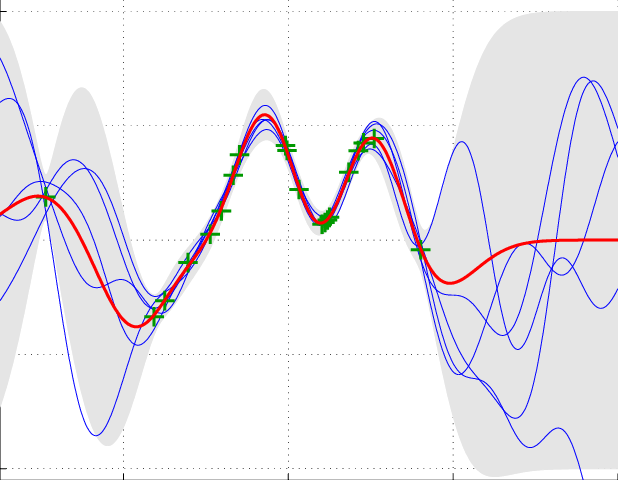
\includegraphics[width=0.4\textwidth]{pictures/files/final/gaussianprocess.png}%
    \caption{\textbf{Mean and variance of a Gaussian process's prediction}. Image from \cite{perez2013gaussian}. Intuitively, variance grows when samples are distant from training samples.}
    \label{fig:gp}%
\end{figure}%

\subsubsection{Discussion of the same norm and low similarity \Cref{ass:inter_sample} on source dataset}
\label{app:discussion_inter_sample}
\Cref{lemma:var_gp} shows that the variance only depends on the input distributions $p(X)$ without involving the label distributions $p(Y|X)$.
This formula highlights that the variance is related to shifts in input similarities (measured by $K$) between $X_{d_S}$ and $X_{d_T}$.
Yet, a more refined analysis of the variance requires additional assumptions, in particular to obtain a closed-form expression of $K(X_{d_S}, X_{d_S})^{-1}$.
\Cref{ass:inter_sample} is useful because then $K(X_{d_S}, X_{d_S})$ is diagonally dominant and can be approximately inverted (see \Cref{app:proof_ood_var}).

The first part of \Cref{ass:inter_sample} assumes that $\exists \lambda_S$ such that all training inputs $x_S\in X_{d_S}$ verify $K(x_S, x_S)= \lambda_S$.
Note that this equality is standard in some kernel machine algorithms \cite{ah2010normalized,ghojogh2021reproducing,rennie2005} and is usually achieved by replacing $K(x,x^\prime)$ by $\lambda_S \frac{K(x,x^\prime)}{\sqrt{K(x,x)}\sqrt{K(x^\prime,x^\prime)}}, \forall(x,x^\prime)\in {(X_{d_S}\cup X_{d_T})}^2$. 
In the NTK literature, this equality is achieved without changing the kernel by normalizing the samples of $X_{d_S}$ such that they lie on the hypersphere; this input preprocessing was used in \cite{Lee2018DeepNN}.
This is theoretically based: for example, the NTK $K(x, x^\prime)$ for an architecture with an initial fully connected layer only depends on $\|x\|,\|x^\prime\|,\langle x, x^\prime\rangle$ \cite{yang2019}. Thus in the case where all samples from $X_{d_S}$ are preprocessed to have the same norm, the value of $K(x_S,x_S)$ does not depend on $x_S\in X_{d_S}$; we denote $\lambda_S$ the corresponding value.

The second part of \Cref{ass:inter_sample} states that $\exists 0 \leq \epsilon \ll \lambda_S, \text{s.t.~} \forall x_S, x_S^\prime \in X_{d_S}^2, x_S\neq x_S^\prime \Rightarrow |K(x_S,x_S^\prime)|\leq\epsilon$, \ie that training samples are dissimilar and do not interact.
This diagonal structure of the NTK \cite{Jacot2018}, with diagonal values larger than non-diagonal ones, is consistent with empirical observations from \cite{seleznova2022neural} at initialization.
% at initialization, when the kernel regime is relaxed.
Theoretically, this is reasonable if $K$ is close to the RBF kernel $K_{h}\left(x, x^{\prime}\right)=\exp (-\left\|x-x^{\prime}\right\|_{2}^{2}/h)$ where $h$ would be the bandwidth: in this case, \Cref{ass:inter_sample} is satisfied when training inputs are distant in pixel space.

We now provide an analysis of the variance where the diagonal assumption is relaxed.
Specifically, we provide the sketch for proving an upper-bound of the variance when the NTK has a block-diagonal structure.
This is indeed closer to the empirical observations in \cite{seleznova2022neural} at the end of training, consistently with the local elasticity property of NNs \cite{He2020The}.
We then consider the dataset $d_{S^\prime} \subset d_S$ made of one sample per block, to which \Cref{ass:inter_sample} applies.
As decreasing the size of a training dataset empirically reduces variance \cite{brain1999effect}, the variance of $f$ trained on $d_S$ is upper-bounded by the variance of $f$ trained on $d_{S^\prime}$; the latter is given by applying \Cref{prop:var} to $d_{S^\prime}$.
We believe that the proper formulation of this idea is beyond the scope of this article and best left for future theoretical work.

\subsubsection{Expression of \ood variance}
\label{app:proof_ood_var}

\begin{proposition*}[\ref{prop:var}]
    Given $f$ trained on source dataset $d_S$ (of size $n_S$) with NTK $K$, under \Cref{ass:infinite_width,ass:inter_sample}, the variance on dataset $d_T$ is:%
    \begin{equation*} \tag{\ref{eq:int_var}}
        \mathbb{E}_{x_T\in X_{d_T}}[\varb(x_T)] = \frac{n_S}{2\lambda_S}\text{MMD}^{2}(X_{d_S}, X_{d_T}) + \lambda_T - \frac{n_S}{2\lambda_S}\beta_T + O(\epsilon),%
    \end{equation*}
    with $\text{MMD}$ the empirical Maximum Mean Discrepancy in the RKHS of $K^2(x,y)=(K(x,y))^2$;$\lambda_T \triangleq \mathbb{E}_{x_T \in X_{d_T}} K\left(x_T, x_T\right)$ and $\beta_T \triangleq \mathbb{E}_{(x_T,x_T^\prime)\in X_{d_T}^2, x_T \neq x_T^\prime} K^2\left(x_T, x_T^{\prime}\right)$ the empirical mean similarities resp. measured between identical (\wrt $K$) and different (\wrt $K^2$) samples averaged over $X_{d_T}$.%
\end{proposition*}
\begin{proof}
Our proof is original and is based on the posterior form of GPs in \Cref{lemma:var_gp}.
Given $d_S$, we recall \Cref{eq:var} that states $\forall x\in\X$:
\begin{align*}
    %\bar{\mu}(x) &=K(x, X_{d_S})\left(K_{X_{d_S}, X_{d_S}}+\sigma_{\epsilon}^{2} \mathbb{I}_{n}\right)^{-1} \boldsymbol{y} \\
    \varb(x) =K(x, x)-K(x, X_{d_S})K(X_{d_S}, X_{d_S})^{-1} K(x, X_{d_S})^\intercal.
\end{align*}
Denoting $B=K(X_{d_S},X_{d_S})^{-1}$ with symmetric coefficients $b_{i,j}=b_{j,i}$, then
\begin{equation} \label{eq:inversion}
    \varb(x) = K(x, x)-\sum_{\substack{1 \leq i \leq n_S \\ 1 \leq j \leq n_S}} b_{i, j} K(x, x_S^i) K(x, x_S^j).
\end{equation}

\Cref{ass:inter_sample} states that
$K(X_{d_S}, X_{d_S})=A+H$ where $A=\lambda_S\mathbb{I}_{n_S}$ and $H=(h_{ij})_{\substack{1 \leq i \leq n_S \\ 1 \leq j \leq n_S}}$ with $h_{i,i}=0$ and $\max_{i,j}|h_{i,j}|\leq\epsilon$.

We fix $x_T \in X_{d_T}$ and determine the form of $B^{-1}$ in two cases: $\epsilon=0$ and $\epsilon\neq 0$.

\paragraph{Case when $\epsilon=0$}
We first derive a simplified result, when $\epsilon=0$.

Then, $b_{i,i}=\frac{1}{\lambda_S}$ and $b_{i,j}=0$ \sut
$$
    \varb(x_T)=K(x_T, x_T)-\sum_{x_S\in X_{d_S}} \frac{K(x_T, x_S)^2}{\lambda_S}=K(x,x) - \frac{n_S}{\lambda_S} \mathbb{E}_{x_S\in X_{d_S}}[K^2(x, x_S)]
$$
We can then write:
\begin{align*}
    &\mathbb{E}_{x_T\in X_{d_T}} [\varb(x_T)] = \mathbb{E}_{x_T\in X_{d_T}}[K(x_T, x_T)] - \frac{n_S}{\lambda_S} \mathbb{E}_{x_T\in X_{d_T}}[\mathbb{E}_{x_S\in X_{d_S}}[K^2(x_T, x_S)]] \\
    &\mathbb{E}_{x_T\in X_{d_T}} [\varb(x_T)] = \lambda_T - \frac{n_S}{\lambda_S} \mathbb{E}_{x_S\in X_{d_S}, x_T\in X_{d_T}}[K^2(x_T, x_S)]. \\
\end{align*}
We now relate the second term on the r.h.s. to a MMD distance.
As $K$ is a kernel, $K^2$ is a kernel and its MMD between $X_{d_S}$ and $X_{d_T}$ is per \cite{Gretton2012}:
\begin{align*}
    %\text{MMD}^{2}(X_{d_S}, X_{d_T})=& \frac{1}{n_S(n_S-1)} \sum_{i=1}^{n_S} \sum_{j \neq i}^{n_S} K^2\left({x_S}_{i}, {x_S}_{j}\right)+\frac{1}{n_T(n_T-1)} \sum_{i=1}^{n_T} \sum_{j \neq i}^{n_T} K^2\left({x_T}_{i}, {x_T}_{j}\right) \\ &-\frac{2}{n_S n_T} \sum_{i=1}^{n_S} \sum_{j=1}^{n_T} K^2\left({x_S}_{i}, {x_T}_{j}\right) \\
    \text{MMD}^{2}(X_{d_S}, X_{d_T})= & \mathbb{E}_{x_S \neq x_S^\prime \in X_{d_S}^2}[K^2(x_S, x_S^\prime)]+\mathbb{E}_{x_T \neq x_T^\prime \in X_{d_T}^2}[K^2(x_T, x_T^\prime)]\\
    & \quad -2\mathbb{E}_{x_S\in X_{d_S}, x_T\in X_{d_T}}[K^2(x_T, x_S)].
\end{align*}
Finally, because $\epsilon=0$, $\mathbb{E}_{x_S \neq x_S^\prime \in X_{d_S}^2} K^2\left(x_S, x_S^{\prime}\right)=0$ \sut
\begin{align*}
    \mathbb{E}_{x_T\in X_{d_T}}[\varb(x_T)] &=\frac{n_S}{2\lambda_S}\text{MMD}^{2}(X_{d_S}, X_{d_T}) + \lambda_T\\
    & \quad\quad\quad -\frac{n_S}{2\lambda_S}\Big(\mathbb{E}_{x_T \neq x_T^\prime \in X_{d_T}^2} K^2\left(x_T, x_T^{\prime}\right)+\mathbb{E}_{x_S \neq x_S^\prime \in X_{d_S}^2} K^2\left(x_S, x_S^{\prime}\right)\Big) \\
    &=\frac{n_S}{2\lambda_S}\text{MMD}^{2}(X_{d_S}, X_{d_T}) +\lambda_T-\frac{n_S}{2\lambda_S}\mathbb{E}_{x_T \neq x_T^\prime \in X_{d_T}^2} K^2\left(x_T, x_T^{\prime}\right)\\
    &= \frac{n_S}{2\lambda_S}\text{MMD}^{2}(X_{d_S}, X_{d_T}) + \lambda_T - \frac{n_S}{2\lambda_S}\beta_T.
\end{align*}

We recover the same expression with a $O(\epsilon)$ in the general setting where $\epsilon\neq 0$.

%DO NOT DELETE
% old version with diagonal error
% \begin{align*}
%     \mathbb{E}_{x\in d_T}[\varb(x)] &=\frac{n_S}{2\lambda}\text{MMD}^{2}(X_{d_S}, X_{d_T}) + \lambda-\frac{n_S}{2\lambda}\Big(\mathbb{E}_{d_T} K^2\left(x_T, x_T^{\prime}\right)+\mathbb{E}_{d_S} K^2\left(x_S, x_S^{\prime}\right)\Big) \\
%     &=\frac{n_S}{2\lambda}\text{MMD}^{2}(X_{d_S}, X_{d_T}) +\lambda-\frac{n_S}{2\lambda}\mathbb{E}_{d_T} K^2\left(x_T, x_T^{\prime}\right)-\frac{n_S}{2\lambda}\mathbb{E}_{d_S} K^2\left(x_S, x_S^{\prime}\right) \\
%     &= \frac{n_S}{2\lambda}\text{MMD}^{2}(X_{d_S}, X_{d_T}) + \lambda - \frac{n_S}{2\lambda}\beta_T-\frac{n_S}{2\lambda} \frac{\lambda^2 n_S}{n_S^2} \\
%     &= \frac{n_S}{2\lambda}\text{MMD}^{2}(X_{d_S}, X_{d_T}) + \lambda - \frac{n_S}{2\lambda}\beta_T-\frac{n_S}{2\lambda} \frac{\lambda^2}{n_S}\\
%     &= \frac{n_S}{2\lambda}\text{MMD}^{2}(X_{d_S}, X_{d_T}) + \lambda - \frac{n_S}{2\lambda}\beta_T-\frac{\lambda}{2}\\
%     &= \frac{n_S}{2\lambda}\text{MMD}^{2}(X_{d_S}, X_{d_T}) + (\frac{\lambda}{2} - \frac{n_S}{2\lambda}\beta_T)
% \end{align*}
% We recover the same expression with a $O(\epsilon)$ in the general setting where $\epsilon\neq 0$.

%DO NOT DELETE
% \paragraph{Case when $\epsilon\neq0$}
% Now, we assume that $\epsilon \neq 0$.
% \Cref{ass:inter_sample} states that
% $$
%     K(X_{d_S}, X_{d_S}) = A + b c^\intercal \text{~where~} A=(1-\epsilon) \mathbb{I}_{n_S}, b=c\triangleq[\sqrt{\epsilon}, \cdots, \sqrt{\epsilon}]^\intercal \in \mathbb{R}^{n_S}
% $$

% We apply Sherman-Morrison to perform inversion:
% \begin{align*}
%     \left(\mathbf{A}+\mathbf{b} \mathbf{c}^{T}\right)^{-1}&=\mathbf{A}^{-1}-\frac{\mathbf{A}^{-1} \mathbf{b} \mathbf{c}^{T} \mathbf{A}^{-1}}{1+\mathbf{c}^{T} \mathbf{A}^{-1} \mathbf{b}} \\
%     &= \frac{1}{1-\epsilon} \mathbb{I}_{n_S}- \frac{1}{1+\frac{\epsilon}{1-\epsilon}n_S}\frac{\epsilon}{(1-\epsilon)}\mathbf{1}_{n_S} \\
%     &=\frac{1}{1-\epsilon} \mathbb{I}_{n_S}- \frac{\epsilon}{1+\epsilon (n_S-1)}\mathbf{1}_{n_S} \\
%     &= (\frac{1}{1-\epsilon}-\frac{\epsilon}{1-\epsilon + \epsilon n_S})\mathbb{I}_{n_S}- \frac{\epsilon}{1-\epsilon + \epsilon n_S}(\mathbf{1}_{n_S}-\mathbb{I}_{n_S})
% \end{align*}
% Therefore, \Cref{eq:inversion} can be developed using $b_{i,i}=\frac{1}{1-\epsilon}-\frac{\epsilon}{1-\epsilon + \epsilon n_S}$ and $b_{i,j}=- \frac{\epsilon}{1-\epsilon + \epsilon n_S}=O(\epsilon)$ and denoting $\frac{1}{\kappa_{\lambda_S,\epsilon}}=b_{i,i}> 0$ into:
% \begin{align*}
%     \varb(x)&=K(x, x)-\sum_{x_S\in X_{d_S}} \frac{K(x, x_S)^2}{\kappa_{\lambda_S,\epsilon}} + O(\epsilon) \\
%     \mathbb{E}_{d_S} [\varb(x)]&= K(x,x)-\mathbb{E}_{d_S}[ \frac{1}{\kappa_{\lambda_S,\epsilon}} \sum_{x_S\in X_{d_S}} K(x, x_S)^2] + O(\epsilon) \\
%     &= K(x,x)-\frac{1}{\kappa_{\lambda_S,\epsilon}}\mathbb{E}_{x_S\sim p_S(X)}[K(x, x_S)^2] + O(\epsilon)
% \end{align*}
% As for the case $\epsilon=0$, we obtain:
% \begin{align*}
%     &\mathbb{E}_{x\in d_T}[\varb(x)] \\
%     &=\frac{1}{2\kappa_{\lambda_S,\epsilon}}\text{MMD}^{2}(X_{d_S}, X_{d_T}) + \mathbb{E}_{x_T\in X_{d_T}} K(x_T, x_T) -\frac{1}{2\kappa_{\lambda_S,\epsilon}}\Big(\mathbb{E}_{p_T(X)} K^2\left(x_T, x_T^{\prime}\right)+\mathbb{E}_{x_S\in X_{d_S}} K^2\left(x_S, x_S^{\prime}\right)\Big) + O(\epsilon)\\
%     &=\frac{1}{2\kappa_{\lambda_S,\epsilon}}\text{MMD}^{2}(X_{d_S}, X_{d_T}) + 1-\frac{1}{2\kappa_{\lambda_S,\epsilon}} 2 {\lambda}^2 + O(\epsilon) \\
%     &= \frac{1}{2\kappa_{\lambda_S,\epsilon}}\text{MMD}^{2}(X_{d_S}, X_{d_T}) + (1-\frac{1^2}{\kappa_{\lambda_S,\epsilon}}) + O(\epsilon)
% \end{align*}
% Moreover, as $\frac{1}{\kappa_{\lambda_S,\epsilon}}=\frac{1}{1-\epsilon}-\frac{\epsilon}{1-\epsilon + \epsilon n_S}$,
% \begin{align*}
%     1-\frac{1^2}{\kappa_{\lambda_S,\epsilon}} = 1 - \frac{1^2}{1-\epsilon} + O(\epsilon) = -\frac{\epsilon1}{1-\epsilon} + O(\epsilon) = O(\epsilon)
% \end{align*}
% Therefore
% $$
%     \mathbb{E}_{x\in d_T}[\varb(x)] = \frac{1}{2\kappa_{\lambda_S,\epsilon}}\text{MMD}^{2}(X_{d_S}, X_{d_T}) + O(\epsilon)
% $$
% where $\frac{1}{\kappa_{\lambda_S,\epsilon}} \rightarrow 1$ when $\epsilon \rightarrow 0$.

\paragraph{Case when $\epsilon\neq 0$}
We denote
$I:\left\{\begin{array}{cl}\mathrm{GL}_{n_S}(\mathbb{R}) & \rightarrow \mathrm{GL}_{n_S}(\mathbb{R}) \\ A & \mapsto A^{-1}\end{array}\right.$
the inversion function defined on $\mathrm{GL}_{n_S}(\mathbb{R})$, the set of invertible matrices of $\mathcal{M}_{n_S}(\mathbb{R})$.

The function $I$ is differentiable \cite{magnus2019matrix} in all $A\in \mathrm{GL}_{n_S}(\mathbb{R})$ with its differentiate given by the linear application
$dI_A:\left\{\begin{array}{cl}\mathcal{M}_{n_S}(\mathbb{R})&\rightarrow \mathcal{M}_{n_S}(\mathbb{R}) \\ H &\mapsto - A^{-1}HA^{-1}\end{array}\right.$. Therefore, we can perform a Taylor expansion of $I$ at the first order at $A$:
\begin{align*}
    I(A+H)&=I(A)+dI_A(H)+o(\|H\|), \\
    (A+H)^{-1}&=A^{-1}-A^{-1}HA^{-1}+o(\|H\|).
\end{align*}
where $\|H\|\leq n_S\epsilon=O(\epsilon)$. Thus,
\begin{align*}
    (\lambda_S\mathbb{I}_{n_S}+H)^{-1}&=(\lambda_S\mathbb{I}_{n_S})^{-1}-(\lambda_S\mathbb{I}_{n_S})^{-1}H(\lambda_S\mathbb{I}_{n_S})^{-1}+O(\epsilon) =\frac{1}{\lambda_S}\mathbb{I}_{n_S}-\frac{1}{\lambda_S^2}H+O(\epsilon), \\
    \forall i \in \llbracket1, n_S\rrbracket, b_{ii}&=\frac{1}{\lambda_S}-\frac{1}{\lambda_S^2}h_{i,i}+o(\epsilon)=\frac{1}{\lambda_S}+O(\epsilon), \\
    \forall i \neq j \in \llbracket1, n_S\rrbracket, b_{ij}&=-\frac{1}{\lambda_S^2}h_{i,j}+o(\epsilon)=O(\epsilon).
\end{align*}

Therefore, when $\epsilon$ is small, \Cref{eq:inversion} can be developed into:
\begin{align*}
    \varb(x_T)&=K(x_T, x_T)-\sum_{x_S\in X_{d_S}} (\frac{1}{\lambda_S}+O(\epsilon)) K(x_T, x_S)^2 + O(\epsilon) \\
    &= K(x_T,x_T)- \frac{n_S}{\lambda_S} \mathbb{E}_{x_S\in X_{d_S}}[K(x_T, x_S)^2] + O(\epsilon)
\end{align*}
Following the derivation for the case $\epsilon=0$, and remarking that under \Cref{ass:inter_sample} we have $\mathbb{E}_{x_S \neq x_S^\prime \in X_{d_S}^2} K^2\left(x_S, x_S^{\prime}\right)=O(\epsilon^2)$, yields:
\begin{equation*}
    \mathbb{E}_{x_T\in X_{d_T}}[\varb(x_T)] = \frac{n_S}{2\lambda_S}\text{MMD}^{2}(X_{d_S}, X_{d_T}) + \lambda_T - \frac{n_S}{2\lambda_S}\beta_T+ O(\epsilon).
\end{equation*}

% When $\lambda=\frac{n_S}{2}$,
% $$
%     \mathbb{E}_{x\in d_T}[\varb(x)] = \text{MMD}^{2}(X_{d_S}, X_{d_T}) + (\frac{n_S}{4} - \beta_T)+ O(\epsilon)
% $$

% Finally, $\beta_T = \frac{\lambda^2 n_T + \alpha_T}{n_T^2}$ where $\alpha_T=\sum_{x_T \neq x_T^\prime} K^2(x_T, x_T^\prime)$ \sut
% $$
%  \frac{n_S}{4} - \beta_T = \frac{n_S}{4} - \frac{\frac{n_S^2}{4} n_T}{n_T^2} - \frac{\alpha_T}{n_T^2}= \frac{n_S}{4} - \frac{n_S^2}{4 n_T} - \frac{\alpha_T}{n_T^2} = \frac{n_S}{4}(1-\frac{n_S}{n_T})-\frac{\alpha_T}{n_T^2}
% $$
% denoting $\kappa_T=\frac{\alpha_T}{n_T^2}\geq 0$
% $$
%     \mathbb{E}_{x\in d_T}[\varb(x)] = \text{MMD}^{2}(X_{d_S}, X_{d_T}) - \frac{n_S}{4}(\frac{n_S}{n_T}-1) - \kappa_T + O(\epsilon)
% $$
\end{proof}

% \begin{lemma}\label{lemma:var_mmd0}
%     When $p_S=p_T$, $\mathbb{E}_{x_T\in X_{d_T}}[\varb(x_T)] = \lambda_T + O(\epsilon)$
% \end{lemma}
% \begin{proof}
%     When $p_S=p_T$, $\text{MMD}^{2}(X_{d_S}, X_{d_T})=0$. The $p_S=p_T$ condition also constrains that $T$ also verifies \Cref{ass:inter_sample} thus $\beta_T=O(\epsilon)$.
%     In conclusion, $\lambda_T$ is the only term left from \Cref{prop:var}.
% \end{proof}
% We recover that variance is small in \iid for infinitely large networks \cite{neal2018modern,belkin2019reconciling,pmlr-v119-d-ascoli20a}.
% \begin{proof}
%     \begin{align*}
%         \mathbb{E}_{x_T\in X_{d_T}} [\varb(x_T)] &= \frac{\lambda}{2} - \frac{n_S}{\lambda} \mathbb{E}_{x_S\in X_{d_S}, x_T\in X_{d_T}}[K^2(x_T, x_S)] + O(\epsilon)\\
%         &=\frac{n_S}{4} -2\mathbb{E}_{x_S\in X_{d_S}, x_T\in X_{d_T}}[K^2(x_T, x_S)]+O(\epsilon)
%     \end{align*}
%     \begin{align*}
%         \text{MMD}^{2}(X_{d_S}, X_{d_T}) &=\mathbb{E}_{X_{d_S}} K^2\left(x_S, x_S^{\prime}\right)+\mathbb{E}_{X_{d_T}} K^2\left(x_T, x_T^{\prime}\right)-2 \mathbb{E}_{X_{d_S}, X_{d_T}} K^2(x_S, x_T) \\
%         &= \frac{\lambda^2 n_S + O(\epsilon^2)}{n_S^2}  + \frac{\lambda^2 n_T}{n_T^2} + \kappa_T -2 \mathbb{E}_{X_{d_S}, X_{d_T}} K^2(x_S, x_T) \\
%         &= \frac{\lambda^2}{n_S}  + \frac{\lambda^2 n_T}{n_T^2} + \kappa_T -2 \mathbb{E}_{X_{d_S}, X_{d_T}} K^2(x_S, x_T) + O(\epsilon^2) \\
%         &= \frac{n_S}{4}  + \frac{n_S^2}{4n_T} + \kappa_T -2 \mathbb{E}_{X_{d_S}, X_{d_T}} K^2(x_S, x_T) + O(\epsilon^2)
%     \end{align*}
%     When $\text{MMD}^{2}(X_{d_S}, X_{d_T})=0$,
%     \begin{align*}
%         -\frac{n_S}{4} - \frac{n_S^2}{4n_T} - \kappa_T  + O(\epsilon^2) = -2 \mathbb{E}_{X_{d_S}, X_{d_T}} K^2(x_S, x_T)
%     \end{align*}
%     \begin{align*}
%         \mathbb{E}_{x_T\in X_{d_T}} [\varb(x_T)] &=  \frac{n_S}{4} -\frac{n_S}{4} - \frac{n_S^2}{4n_T} - \kappa_T  + O(\epsilon^2) \\
%         &= - \frac{n_S^2}{4n_T} - \kappa_T  + O(\epsilon^2)
%     \end{align*}
% \end{proof}

\subsubsection{Variance and initialization}
\label{remark:mmdk}

The MMD depends on the kernel $K$, \ie only on the initialization of $f$ in the kernel regime per \cite{Jacot2018}. Thus, to reduce variance, we could act on the initialization to match $p_S(X)$ and $p_T(X)$ in the RKHS of $K^2$.
This is consistent with \Cref{subsec:expression_ood_bias} that motivated matching the train and test in features.
In our paper, we used the standard pretraining from ImageNet \cite{krizhevsky2012imagenet}, as commonly done on DomainBed \cite{gulrajani2021in}.
The Linear Probing \cite{kumar2022finetuning} initialization of the classifier was shown in \cite{kumar2022finetuning} to prevent the distortion of the features along the training.
This could be improved by pretraining the encoder on a task with fewer domain-specific information, \eg CLIP \cite{radford2021learning} image-to-text translation as in \cite{ruan2022optimal}.
\subsection{WA \versus its members}
\label{app:proof_wa_ind}
We validate that WA's expected error is smaller than its members' error under the locality constraint.
\begin{lemma}[WA \versus its members.]\label{lemma:wa_ind}
    \begin{equation}
        \mathbb{E}_{L_S^M}\mathcal{E}_T(\theta_{\text{WA}}(L_S^M)) - \mathbb{E}_{l_S} \mathcal{E}_T \left(\theta \left( l_S \right) \right)= \frac{M-1}{M} \mathbb{E}_{x\sim p_T}[\covb(x)-\varb(x)] + O(\Deltab^2) \leq O(\bar{\Delta}^2).%
    \end{equation}%
\end{lemma}%
\begin{proof}
    The proof builds upon \Cref{eq:b_var_cov}:
    \begin{equation*}
        \mathbb{E}_{L_S^M}\mathcal{E}_T(\theta_{\text{WA}}) = \mathbb{E}_{(x,y)\sim p_T}\Big[\biasb(x,y)^{2}+\frac{1}{M} \varb(x)+\frac{M-1}{M} \covb(x)\Big] + O(\Deltab^2),
    \end{equation*}
    and the expression of the standard bias-variance decomposition in \Cref{eq:b_v} from \cite{kohavi1996bias},
    \begin{equation*}
        \mathbb{E}_{l_S}\mathcal{E}_T(\theta) = \mathbb{E}_{(x,y)\sim p_T}\Big[\biasb(x,y)^{2}+\varb(x)\Big].
    \end{equation*}
    The difference between the two provides:
    \begin{equation*}
        \mathbb{E}_{L_S^M}\mathcal{E}_T(\theta_{\text{WA}}) - \mathbb{E}_{l_S}\mathcal{E}_T(\theta) = \frac{M-1}{M} \mathbb{E}_{(x,y)\sim p_T} \Big[\covb(x)-\varb(x)\Big] + O(\Deltab^2).
    \end{equation*}
    Cauchy Schwartz inequality states $|\mathrm{cov}(Y, Y')| \leq \sqrt{\mathrm{var}(Y) \mathrm{var}(Y')}$, thus $\covb(x)\leq\varb(x)$. Then:
    \begin{equation*}
        \mathbb{E}_{L_S^M}\mathcal{E}_T(\theta_{\text{WA}}) - \mathbb{E}_{l_S}\mathcal{E}_T(\theta) \leq O(\Deltab^2).
    \end{equation*}
\end{proof}
